\documentclass{beamer}
\usepackage{hyperref}
\usepackage{subfig}  %% Para incluir subgraficos
\usepackage{graphicx}
\usepackage{media9} % 
\usepackage{url}
\usepackage{ragged2e}  % Allow justification
\usepackage[margin=20pt,font=small,labelfont=bf,labelsep=period]{caption}

\usepackage[spanish, activeacute]{babel}
\usepackage[utf8]{inputenc}
\decimalpoint
%\usepackage{natbib}

%
\hypersetup{pdfstartview={Fit}, bookmarks=True, pdftitle={SCEC Presentation}, pdfauthor={Juan Carlos Vergara-Gallego}, pdfsubject={Presentation}, pdfkeywords={Waves, Elasticity, Numerical Methods, High Performance Computing, BEM}, pdfpagemode=UseOutlines, bookmarks, bookmarksopen, pdfstartview=FitH, colorlinks,linkcolor=blue, urlcolor=black, citecolor=blue}  % Configure hyperref

%--- New commands ----%
\newcommand{\footref}[1]{\textsuperscript{\ref{#1}}}
\newcommand{\pardiff}[2]{\frac{\partial #1}{\partial #2}}
\newcommand{\pardiffd}[2]{\frac{\partial^2 #1}{\partial #2^2}}
%
%---------------------%
%\usefonttheme[onlymath]{serif}  % Make equations to be in serif fonts
\usefonttheme{serif}  % Make equations to be in serif fonts

\begin{document}


%title
\title[CyberShake] % (optional, only for long titles)
{A Physics-Based Seismic Hazard Model for Southern California}
\subtitle{CyberShake, Southern California Earthquake Center}
\author[Vergara Gallego, Juan Carlos] % (optional, for multiple authors)
{Juan Carlos Vergara Gallego\\ \texttt{\small jvergar2@eafit.edu.co}\\
{\tiny Presentación disponible en: \url{https://github.com/jvergar2/03_SCEC}}}
\institute{Departamento de Ingeniería Civil\\
  Universidad EAFIT}
\date{\today}
\subject{Ingeniería Sísmica}

% Title page
\frame{\titlepage}

% Outline
\begin{frame}
	\frametitle{Outline}
	\tableofcontents
\end{frame}
%
%
\section{Introduction}
\begin{frame}
\frametitle{Introducción}
%
\justifying
Se presenta un resumen del proyecto {C}yber{S}hake, de sus objetivos y la foma como están abordando el problema de construir el modelo de Amenaza en el Sur de California.

\url{http://scec.usc.edu/scecpedia/CyberShake}
%
\end{frame}
%
%
\begin{frame}[allowframebreaks]
\frametitle{¿Qué es el CyberShake?}
%
\justifying
{C}yber{S}hake, es un proyecto de investigación del ``Southern California Earthquake Center's" (SCEC), dentro del cual se encuentran desarrollando un modelo computacional a gran escala para incluir determinísticamente el efecto de la fuente y la ruta de propagación de las ondas sísmicas en la amenaza sísmica del Sur de California.
%
\end{frame}
%\transwipe
%
\begin{frame}
\frametitle{¿Qué es el CyberShake?}
\begin{figure}[h]
	\centering
	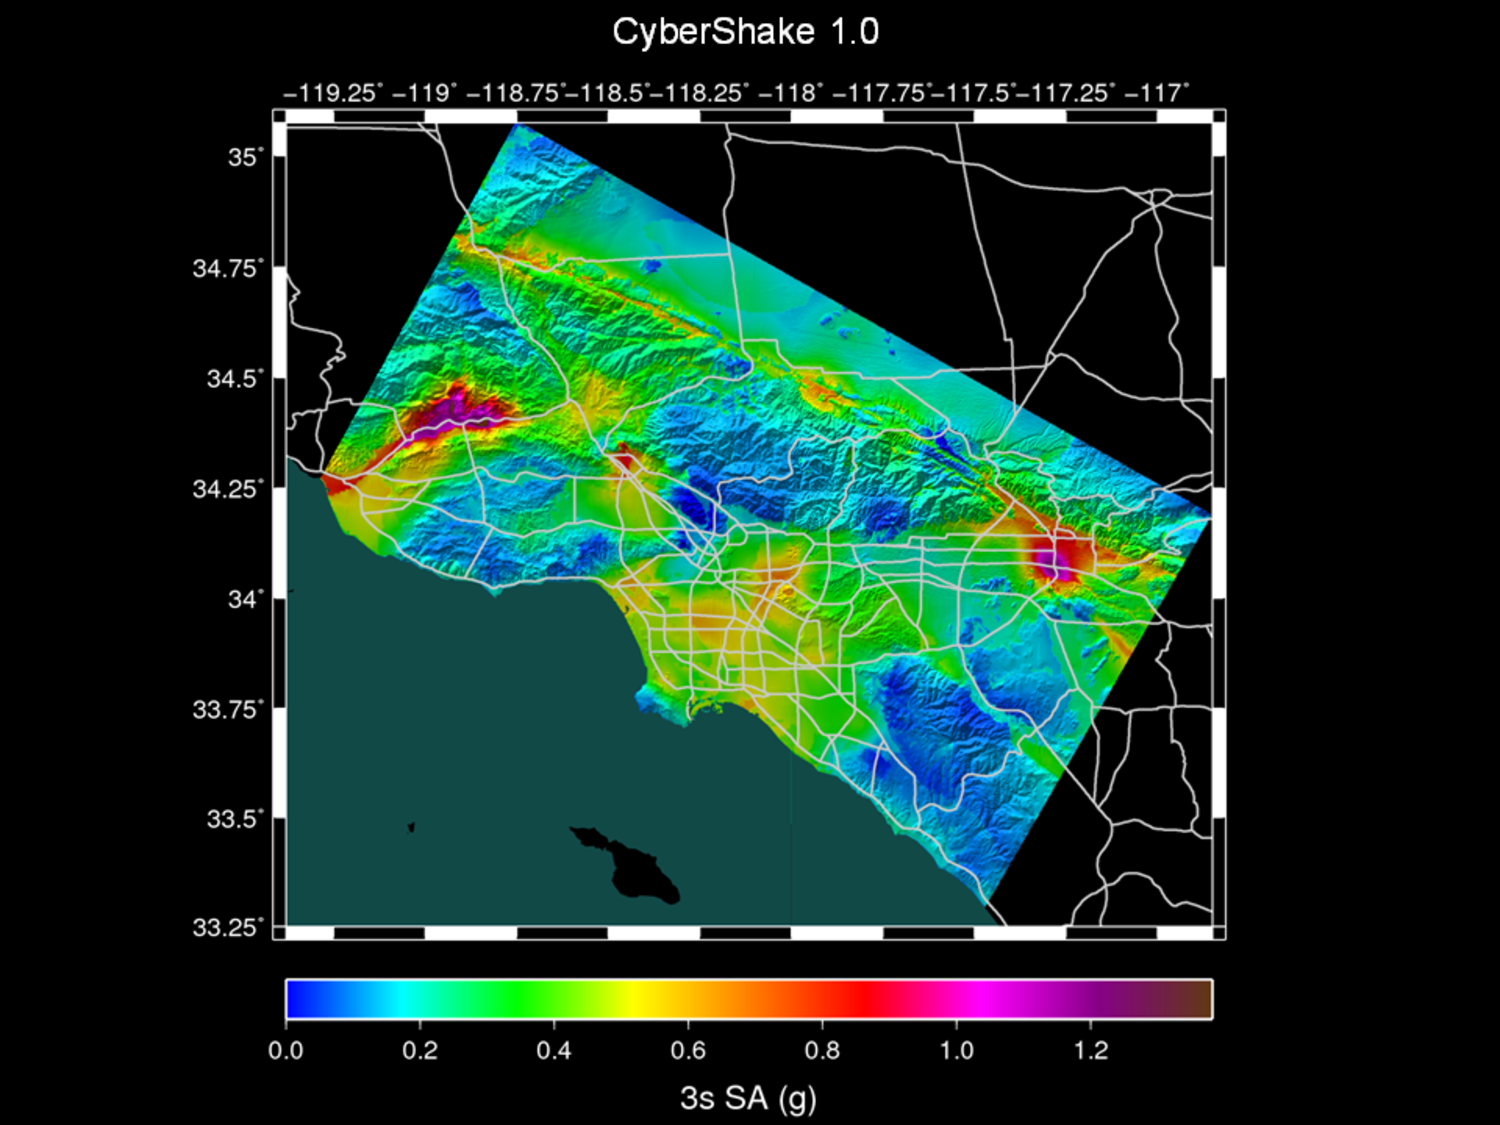
\includegraphics[height=6cm]{img/CyberShake_2009.pdf}
	\caption{Mapa de amenaza sísmica del Sur de California calculado con CyberShake. \footnote{\tiny \url{http://scec.usc.edu/scecwiki/images/6/61/CandB_2008.PNG}\\}}
\end{figure} 
%
\end{frame}
%
%
\begin{frame}
\frametitle{¿Qué es el CyberShake?}
%
\begin{figure}[h]
	\centering
	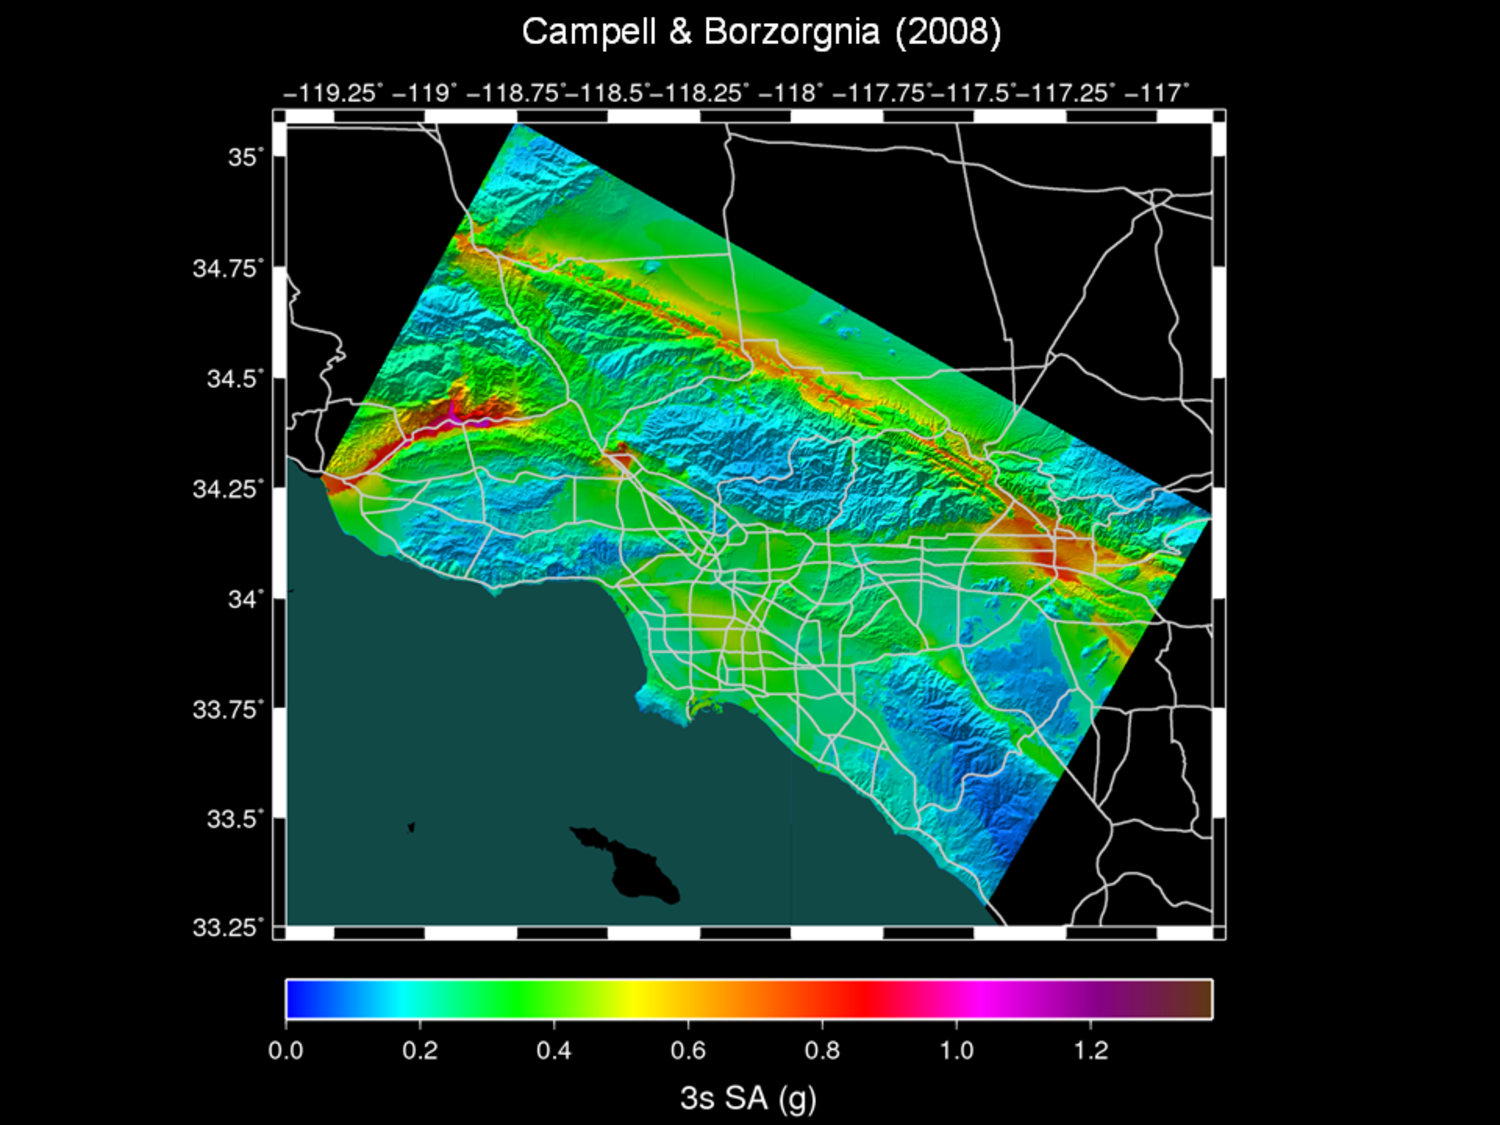
\includegraphics[height=6cm]{img/CandB_2008.pdf}
	\caption{Mapa de amenaza sísmica del Sur de California calculado con las ecuaciones de predición del movimiento del suelo (GMPE). \footnote{\tiny \url{http://scec.usc.edu/scecwiki/images/6/61/CandB_2008.PNG}\\}}
\end{figure}
%
%
%\begin{figure}[h]
%\centering
%%
%	\subfloat[Ricker pulse.]{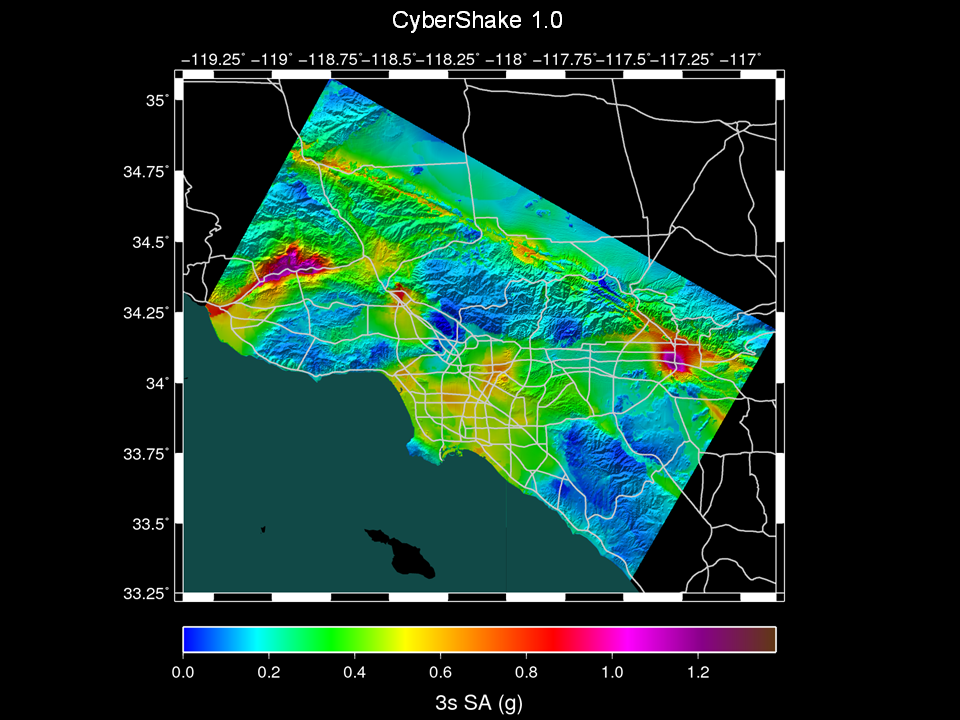
\includegraphics[width=0.4\textwidth]{img/CyberShake_2009.PNG}}\qquad
%	%
%	\subfloat[Ricker pulse spectrum.]{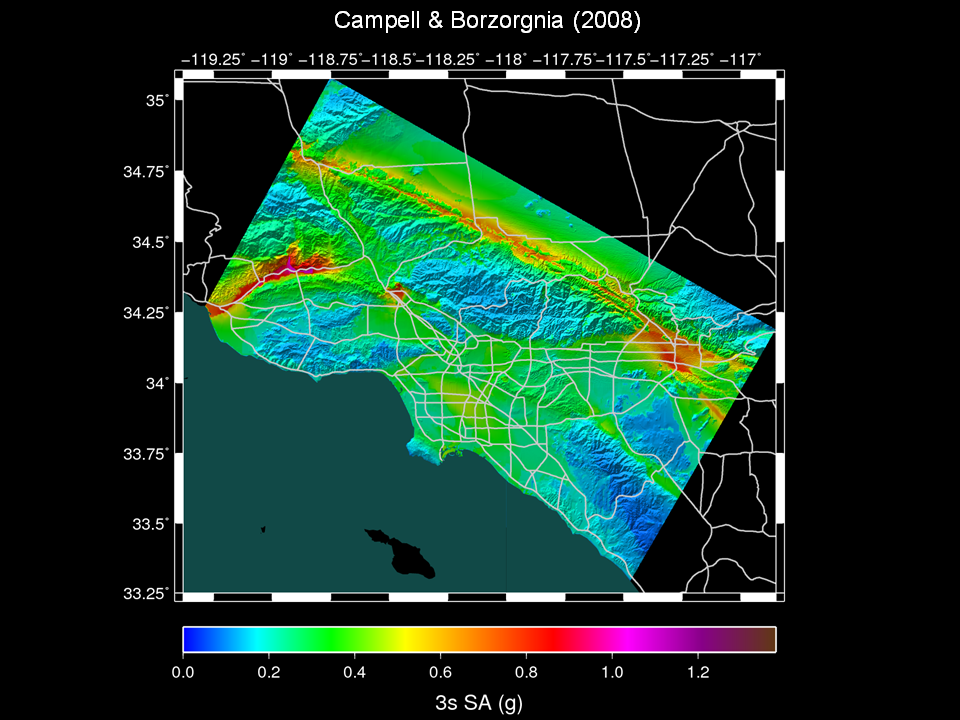
\includegraphics[width=0.4\textwidth]{img/CandB_2008.PNG}}
%	%
%\caption{Ricker pulse and its spectrum.}
%
%\end{figure}
\end{frame}
%
%
\section{¿Qué se hace actualmente?}
\begin{frame}[allowframebreaks]\frametitle{Ground Motion Prediction Equations}
%
\justifying
Las Ecuaciones de Predicción del Movimiento Sísmico del Suelo (GMPEs), especifican la probabilidad de excedencia del movimiento del suelo en un sitio particular para una fuente específica representada por un escenario de ruptura específico.\\
%
Las GMPEs entregan $S_a \left( T \right)$ para el $5\%$ de amortiguamiento.
%
\begin{figure}[h]
	\centering
	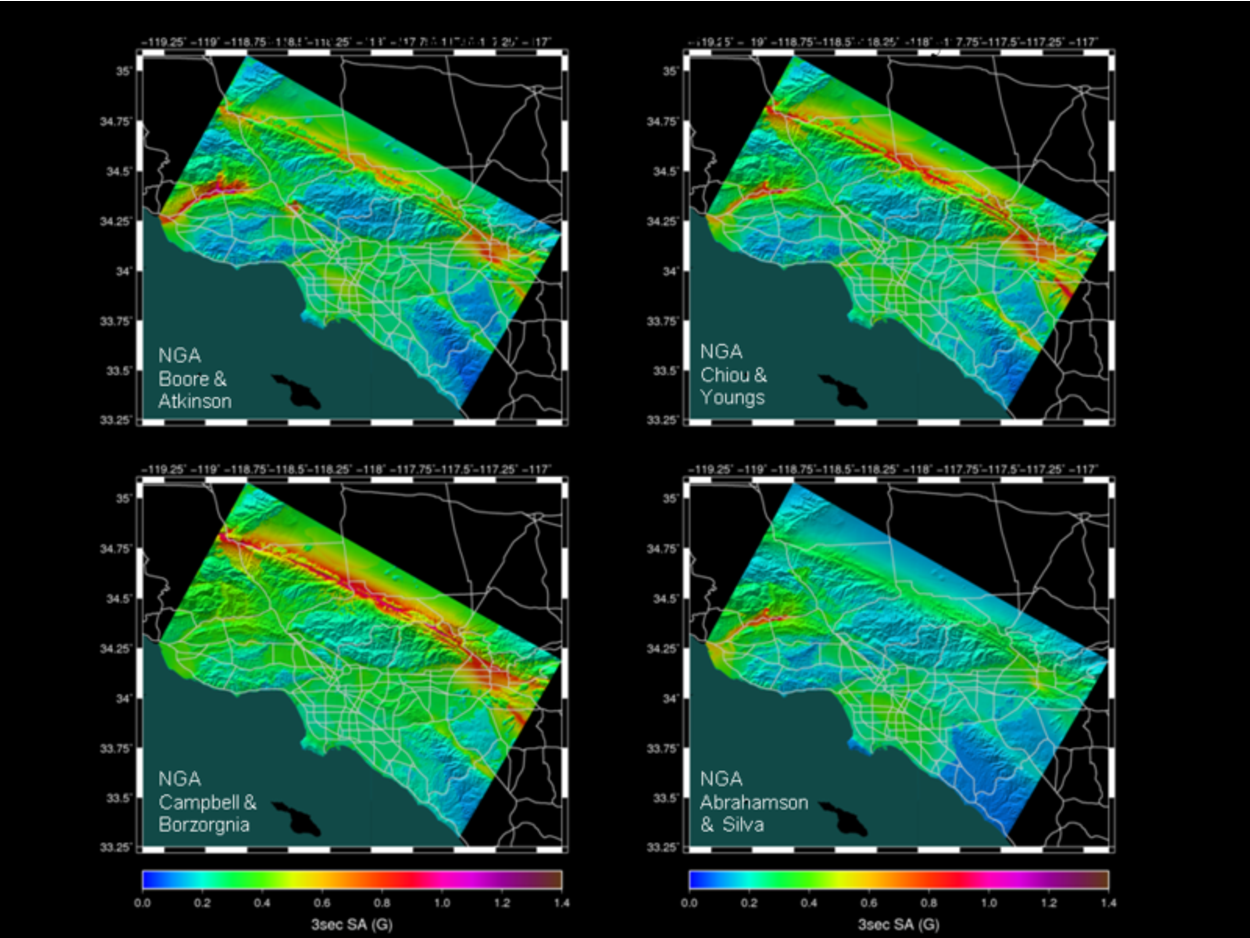
\includegraphics[height=3cm]{img/UCERF2_GMPE_2007.pdf}
	\caption{Mapa de amenaza sísmica del Sur de California calculado con cautro ecuaciones de predición del movimiento del suelo (GMPE) diferentes. \footnote{ \tiny\url{http://scec.usc.edu/scecwiki/images/b/bd/UCERF2_GMPE_2007.PNG}\\}}
\end{figure}
%
\justifying
A pesar de que las cuatro leyes de atenuación son aceptadas en la comunidad científica, es evidente las grandes diferencias entre ellas.\\
%
%
\end{frame}
%
%
\section{¿Con que información cuentan?}
\subsection{UCERF $2.0$ y $3.0$}
\begin{frame}[allowframebreaks]
\frametitle{Uniform California Earthquake Rupture Forecast, Version $2.0$ y $3.0$ (UCERF $2.0$ y $3.0$)}
%
\justifying
%
El $UCERF3.0$ estima la probabilidad de ocurrencia de sismos, para una magnitud específica y localización, que pueden ocurrir dentro de una ventana de tiempo en California EE.UU. La versión $3.0$ es una mejora de la versión $2.0$, dando la posibilidad de la ruptura simultanea de varias fallas y mejorando la sobre-estimación que daba $UCERF2.0$ para magnitudes entre $6.5$ y $7.0$.\\
%
Cuantro componentes básicos de $UCERF3.0$:
%
	\begin{itemize}
	\justifying
	%
		\item Modelo de Falla: Geometría física de las fallas conocidas.
		%
		\item Modelo de Deformación: ``Taza de deslizamiento" de cada sección de la falla. Con esto se calcula el momento sísmico.
		%
		\item ``Earthquake Rate Model": Taza de todos los sismos dentro de una región sobre una magnitud mínima especificada.
		%
		\item Modelos de Probabilidad: Determina la probabilidad de ocurrencia de cada evento dentro de una ventana de tiempo.
	%
	\end{itemize}
%
\begin{figure}[h]
	\centering
	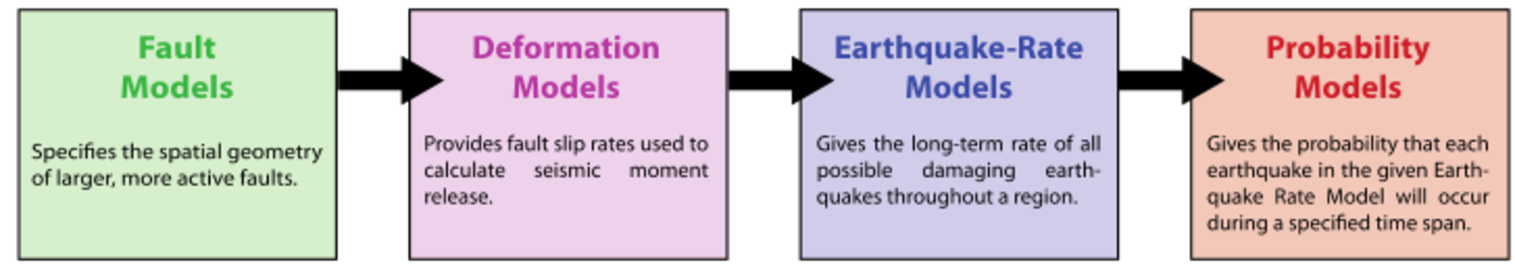
\includegraphics[height=1.75cm]{img/Components_UCERF.pdf}
	\caption{Componentes básicos del modelo UCERF3.0. \cite[figura 2, página 7]{ucerf3}}
\end{figure}
%
%
\justifying
Con la información suministrada por $UCERF2.0$ se identifican todas las posibles fallas sísmicas $200$ $km$ dentro de la región de estudio. Todas las fallas se usan para generar diferentes escenarios, dentro de los cuales se varía la ubicación del hypocentro y la forma de la ruptura.\\
%
En total se generan al rededor de $415.000$ escenarios de ruptura para cada sitio. 
%
%
%\end{frame}
%%
%%
%\begin{frame}[allowframebreaks]
%\frametitle{Uniform California Earthquake Rupture Forecast, Version $2.0$ y $3.0$ (UCERF $2.0$ y $3.0$)}
%
\begin{figure}[h]
	\centering
	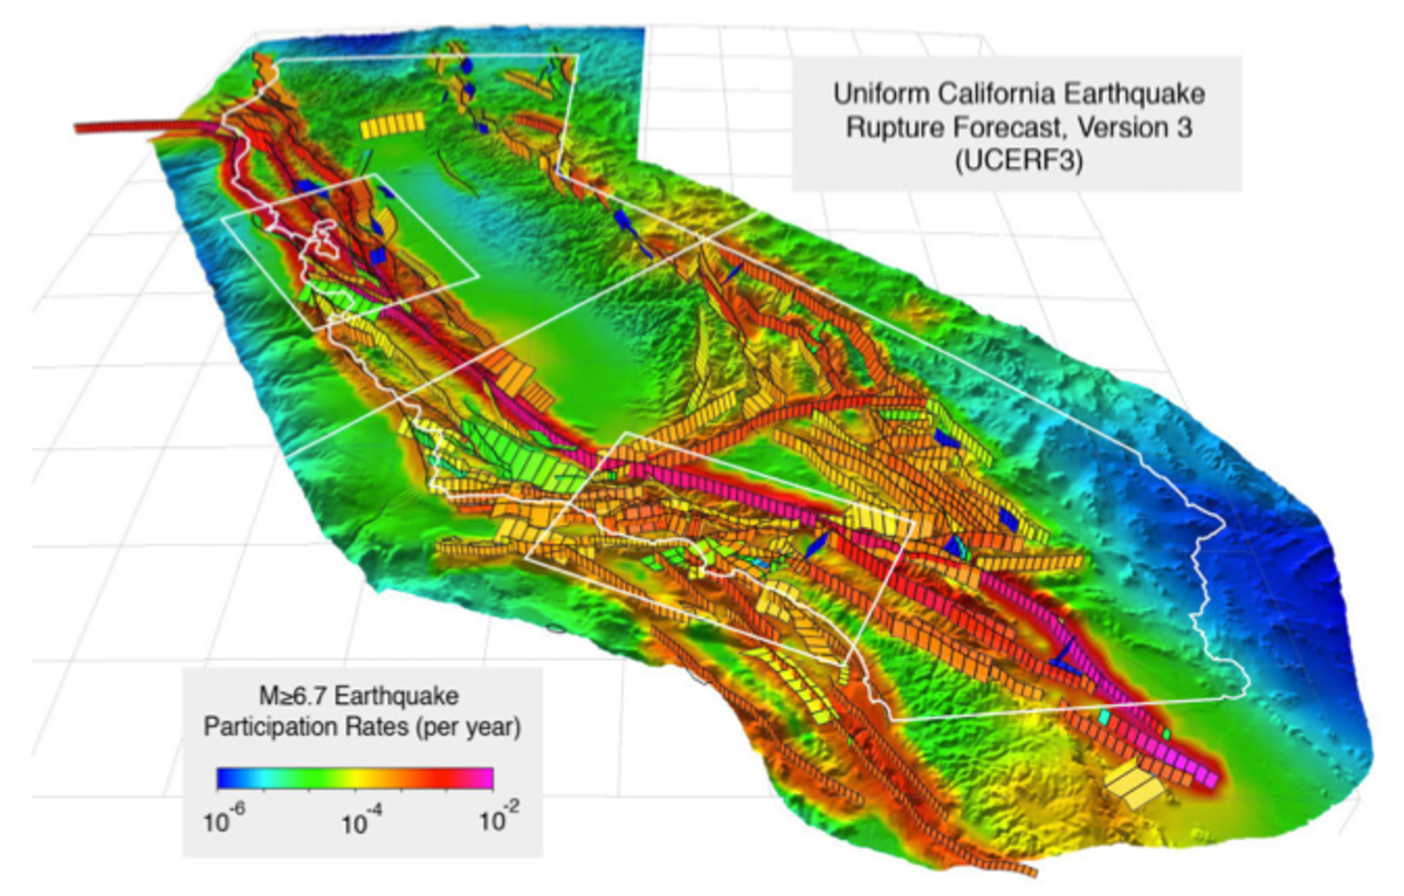
\includegraphics[height=6cm]{img/UCERF3_Map.pdf}
	\caption{Mapa $3D$ de California, mostrando las $2606$ fallas mapeadas en $UCERF3.0$ \cite[figura 1, página 5]{ucerf3}}
\end{figure}
%
\end{frame}
%
%
\subsection{Modelos de Velocidad}
\begin{frame}[allowframebreaks]
\frametitle{SCEC Community Velocity Model: CVM-S.}
%
\justifying
%
El modelo de velocidad comunitario de California (CVM-S \footnote{Actualmente se encuentra disponible en linea la versión $4.0$ de dicho modelo. \url{http://www.data.scec.org/research-tools/3d-velocity.html}, \url{http://scec.usc.edu/scecpedia/CVM-S}, último acceso $03$ de Octubre de $2014$.}, por sus siglas en ingles), tiene como propósito servir como modelo de referencia en varias áreas de investigación que dependen de las estrucutras, propiedades de los materiales tales como la velocidad de propagación de las ondas sísmicas, en profundidad para llevar acabo diferentes análisis. Las velocidades de mayor profundidad se construye con base reglas que relacionan la profundidad y la edad de los depósitos sedimentarios con las velocidades de las ondas sísmicas. Las velocidades de propagación en los depósitos menos profundos son tomadas de las medidas de los estudios geotécnicos. Las velocidades de propagación en roca son tomados de estudios tomográficos.\\
%
El modelo de velocidad CVM-S es de libre acceso, un usuario puede obtener los códigos escritos en Fortran, compilarlos y ejecutarlos en una máquina personal. El código se alimenta con un archivo de texto que contiene la latitud, longitud y profundidad de puntos donde se quiere conocer $V_p$, $V_s$ y $\rho$.
%
%
\begin{figure}[h]
	\centering
	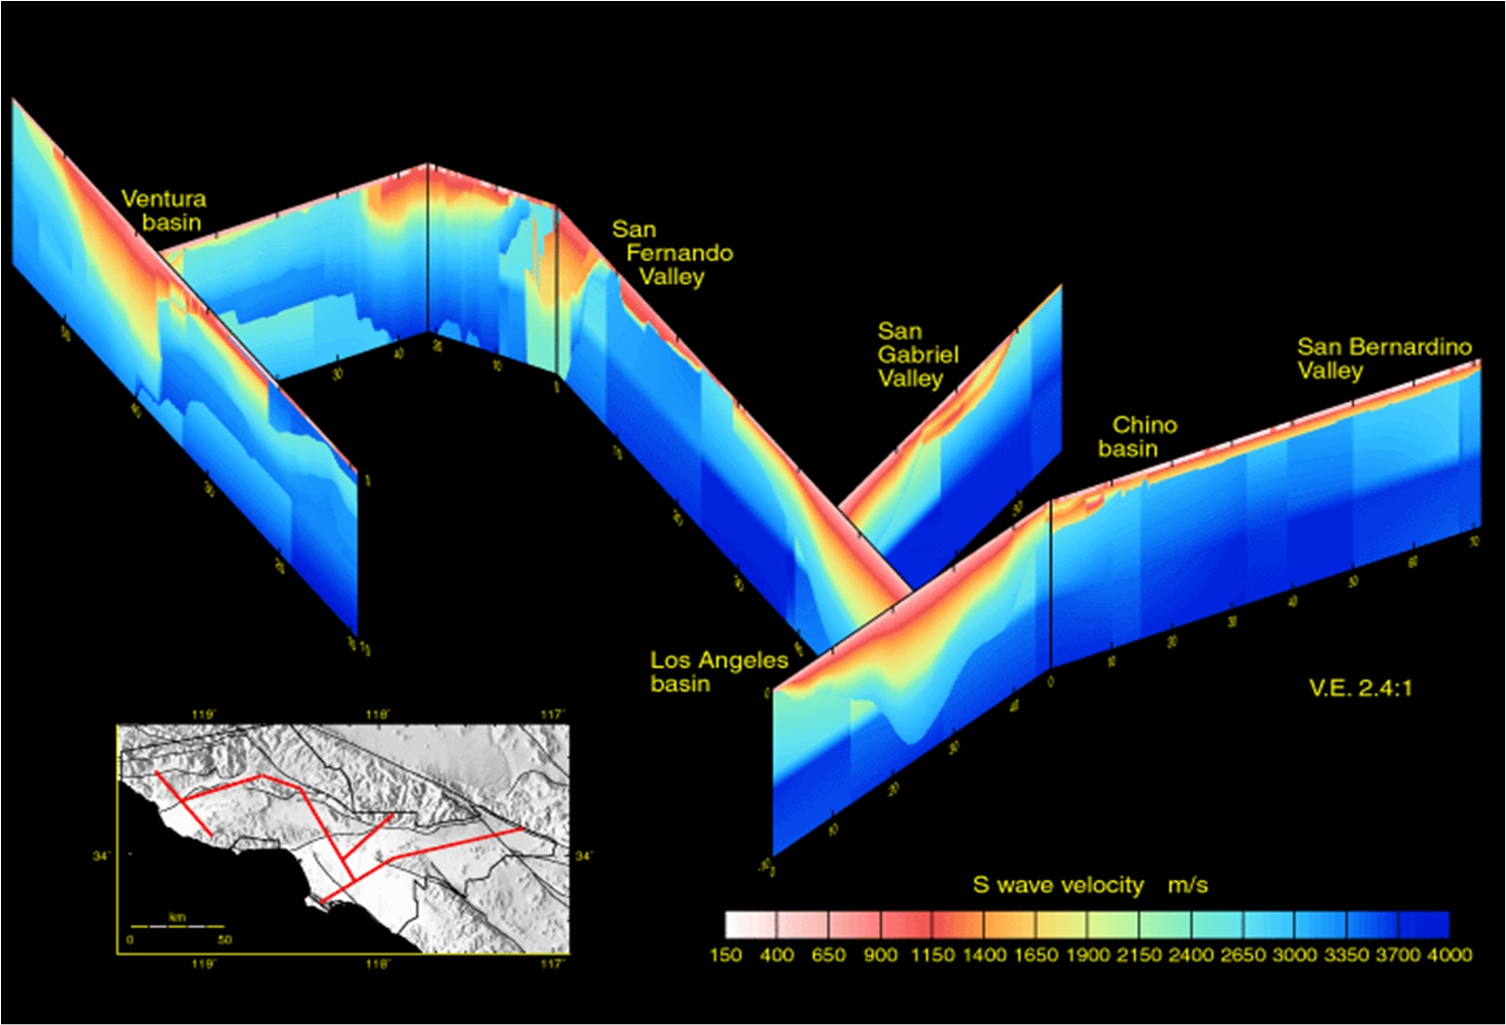
\includegraphics[height=5cm]{img/CVM-S4.pdf}
	\caption{Secciones transversales de California mostrando la variación en profundidad de la velocidad. \footnote{\tiny \url{http://scec.usc.edu/scecwiki/images/a/a7/CVM-S4.png}\\}}
\end{figure}
%
\end{frame}
%
%
\begin{frame}[allowframebreaks]
\frametitle{SCEC Community Velocity Model: CVM-H.}
%
\justifying
%
El Modelo de Velocidad Comunitario - Harvard (CVM-H \footnote{\tiny Actualmente se encuentra disponible en linea la versión $11.9.0$ de dicho modelo. \url{http://scec.usc.edu/scecpedia/CVM-H}}, por sus siglas en ingles), se basa en ensayos de reflexión sísmica y ``Borehole" para la estimación de la velocidad de propagación de la onda sísmica en puntos específicos. Dicha información se interpola en una malla bastante refinada cubriendo toda la región que se quiere estudiar. Adicionalmente contiene una descripción extensiva del modelo de velocidad en la región fuera de la costa (offshore).
%
\begin{figure}[h]
	\centering
	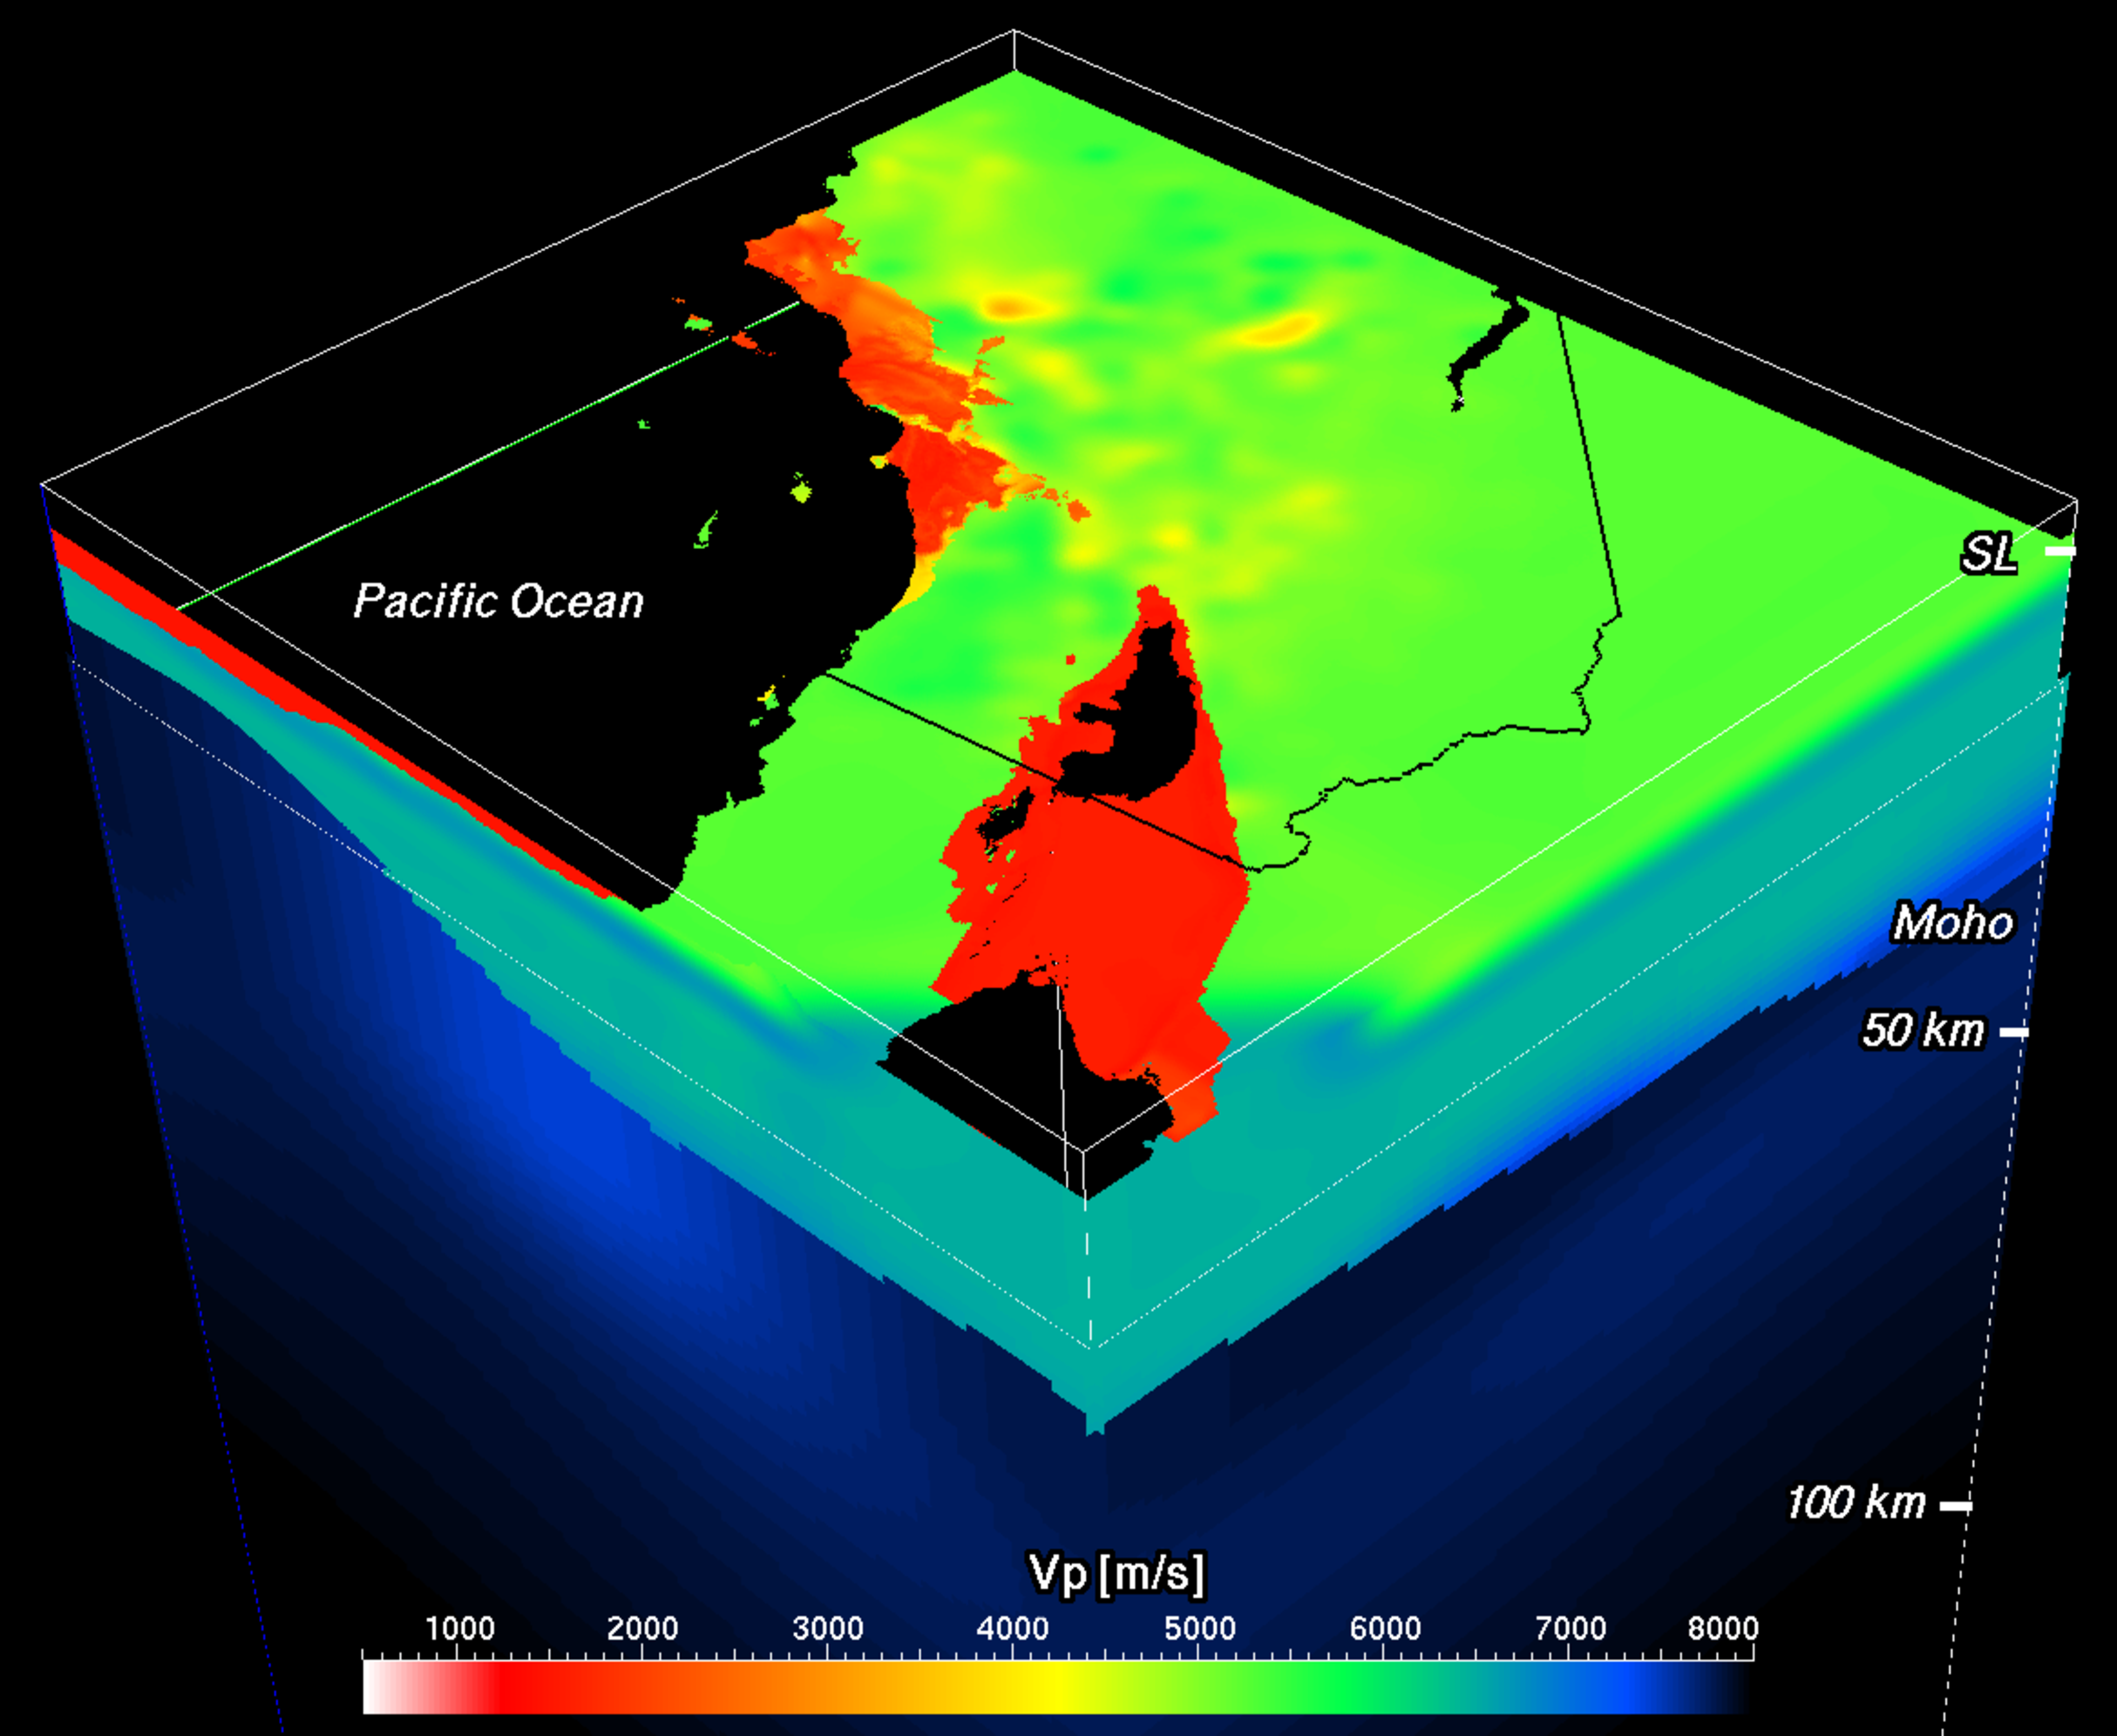
\includegraphics[height=5cm]{img/CVM64_perspectve.pdf}
	\caption{Perspectiva Modelo de Velocidad Comunitario - Harvard (CVM-H). \footnote{\tiny\url{http://scec.usc.edu/scecwiki/images/a/a1/CVM64_perspectve.png}\\}}
\end{figure}
%
%
\end{frame}
%
%
\section{¿Qué hacen y cómo lo hacen?}
\subsection{Objetivos}
\begin{frame}%[allowframebreaks]
\frametitle{Objetivos}
%
\justifying
%
Uno de los objetivos de CyberShake es mejorar las Ecuaciones de Predicción de Movimiento del Suelo (GMPEs), comúnmente usadas en ingeniería.\\
%
El objetivo principal, el objetivo más ambicioso, es remplazar por completo las leyes de atenuación con simulaciones a gran escala para la predicción de los movimientos sísmicos del suelo y con estos calcular los mapas de amenaza sísmica.\\
%
CyberShake se está desarrollando en el Sur de California, pero la metodología se puede aplicar en cualquier región del mundo donde se cuente con la información suficiente y se tengan los recursos computacionales.
%
%
\end{frame}
%
%
\subsection{Modelos Computacionales}
\begin{frame}%[allowframebreaks]
\frametitle{Modelos computacionales}
%
\justifying
%
En un sitio particular, es necesario conocer la incidencia de varios eventos sísmicos, generados por diferentes sismofuentes, para poder generar unas curvas de amenaza sísmica lo suficientemente confiables.\\
%
Teniendo los modelos computacionales a gran escala, es posible generar cuantos eventos sísmicos sean necesarios y tener en cuenta la generación de sismos desde varios tipos de fuentes, tener en cuenta la incidencia de los factores tales como la ruta de propagación de las ondas, los efectos de fuente y sismos de diferentes magnitudes generados por una misma fuente.\\
%
En un sitio particular, CyberShake directamente muestrea la variabilidad del movimiento del suelo a partir de información de varios sismos (escenarios de ruptura) y elimina la necesidad de asumir que los procesos son ergódicos.\\
%
\end{frame}
%
%
\begin{frame}%[allowframebreaks]
\frametitle{Procesos Ergódicos}
%
\justifying
%
\begin{figure}[h]
	\centering
	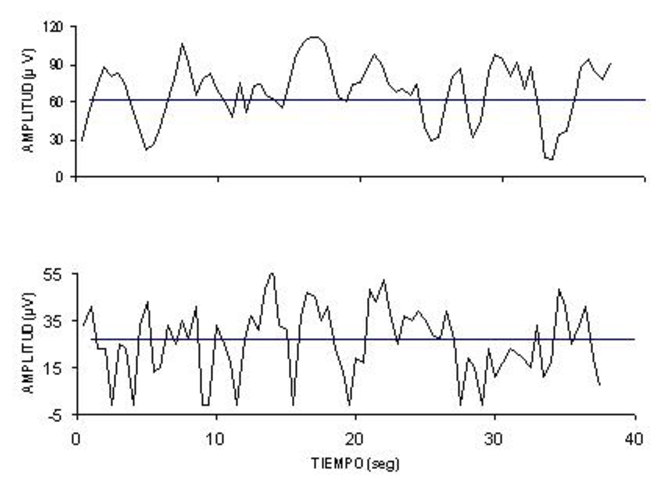
\includegraphics[height=3.5cm]{img/Ergodico.pdf}
	\caption{Definición gráfica de un proceso Ergódico. Imagen tomada de \footnote{\tiny \url{http://www.iga.cu/publicaciones/revista/cte_07/art_07-01/id28.htm}\\}}
\end{figure}
%
\textbf{Proceso Ergódico:} Los promedios o medias hacia la derecha son iguales hacia abajo. Es lo mismo hallar los indicadores de un acelerograma que de varios.\\
%
\end{frame}
%
%
\begin{frame}%[allowframebreaks]
\frametitle{Discretización de la región de estudio}
%
\justifying
\begin{figure}[h]
	\centering
	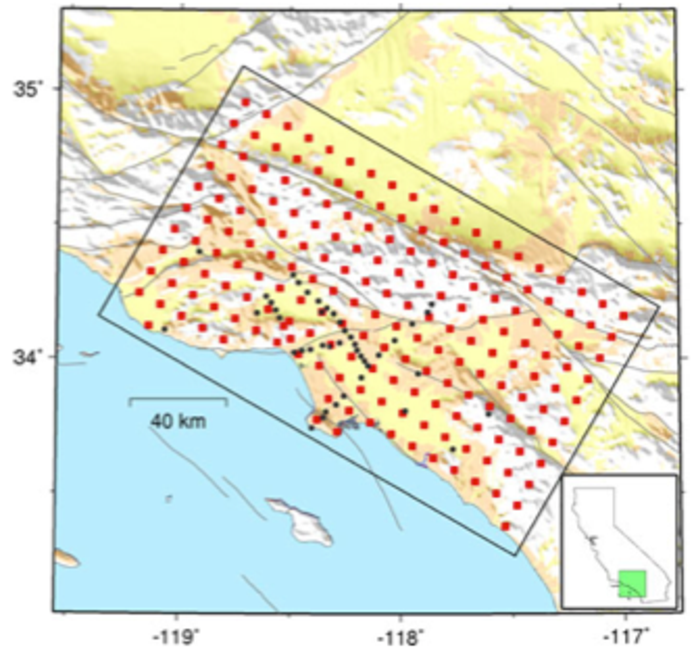
\includegraphics[height=4cm]{img/Discretizacion.pdf}
	\caption{Mapa del Sur de California mostrando los puntos en los cuales se calculan las curvas de amenaza. \cite[figura 1, página 3]{gravesetal}}
	\vspace{-.5 cm}
\end{figure}
%
Dentro del proyecto CyberShake, se han simulado diferentes escenarios de ruptura y se han calculado las curvas de amenaza en $250$ sitios en la región de Los Angeles, con lo cual tienen las bases para la generación de mapas de amenaza sísmica a partir de CyberShake.\\
%
%
\end{frame}
%
%
\begin{frame}[allowframebreaks]
\frametitle{¿Por qué no calcular las curvas de amenaza en los puntos de la malla en superficie?}
%
\justifying
%
Dentro de la región de Los Angeles se tienen identificadas al rededor de $10.000$ fallas que pueden generar sismos de intensidad mayor igual a $6.0$ $(M_w \geq 6.0)$ que pueden afectar la región bajo estudio.
%
\begin{figure}[h]
	\centering
	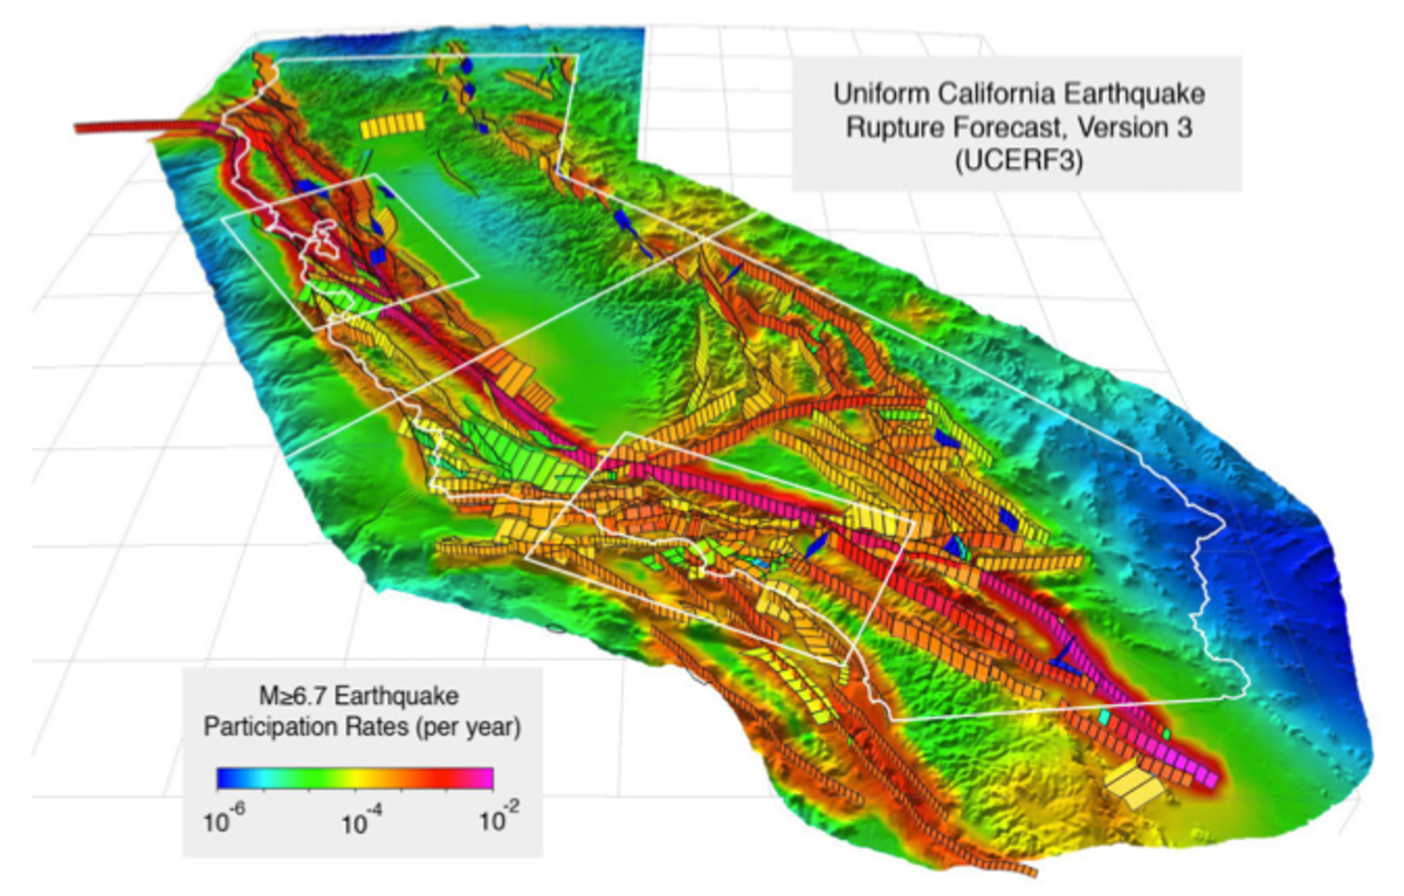
\includegraphics[height=4cm]{img/UCERF3_Map.pdf}
	\caption{Mapa $3D$ de California, mostrando las $10.000$ fallas mapeadas en $UCERF3.0$ \cite[figura 1, página 5]{ucerf3}}
\end{figure}
%
A partir de cada falla se generan diferentes escenarios, donde se varían factores tales como la ubicación del hipocentro, magnitud del evento y proceso de ruptura. Dentro de CyberShake se han generado al rededor de $415.000$ escenarios diferentes.\\
%
\begin{figure}[h]
	\centering
	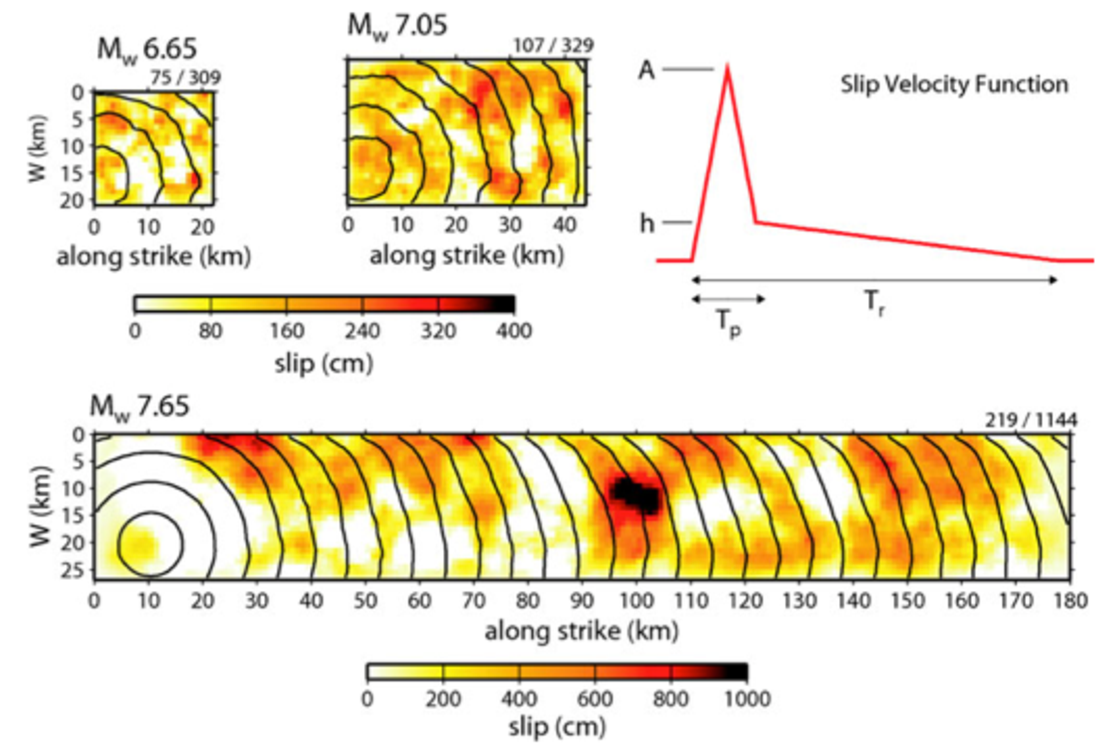
\includegraphics[height=4cm]{img/ModeloRuptura.pdf}
	\caption{Cinemática para diferentes escenarios de ruptura. \cite[figura 4, página 7]{gravesetal}}
\end{figure}
%
Cada escenario diferente representa un modelo computacional diferente, por lo cual sería necesario analizar $415.000$ modelos $3D$ a gran escala con los costos computacionales que esto representa y la cantidad de información que se genera.\\ 
%
%
\end{frame}
%
%
\begin{frame}[allowframebreaks]
\frametitle{¿Cómo se calculan las SGT?}
%
\justifying
%
CyberShake discretiza la región de estudio en $250$ sitios en los cuales se quiere calcular la curva de amenaza, puntos en los cuales se quieren conocer los registros sintéticos.
%
\begin{figure}[h]
	\centering
	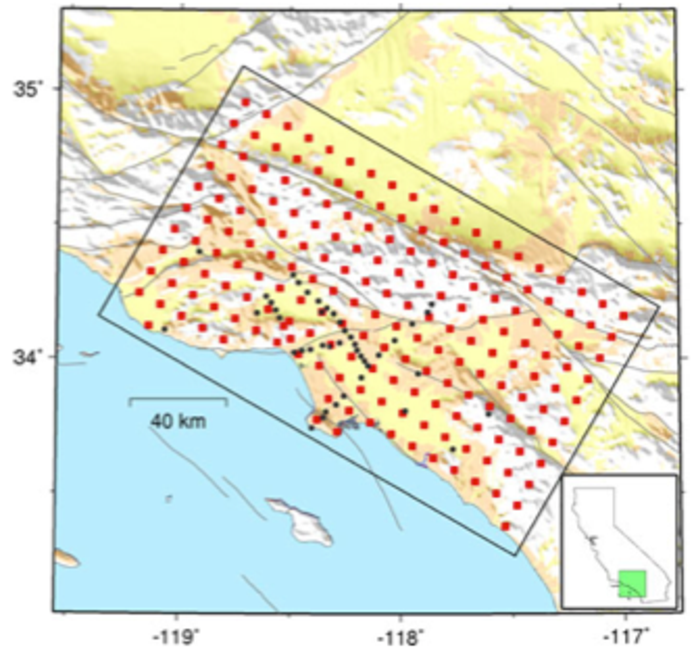
\includegraphics[height=4cm]{img/Discretizacion.pdf}
	\caption{Mapa del Sur de California mostrando los puntos en los cuales se calculan los registros sintéticos. \cite[figura 1, página 3]{gravesetal}}
	\vspace{-.5 cm}
\end{figure}
%
%
\begin{figure}[h]
	\centering
	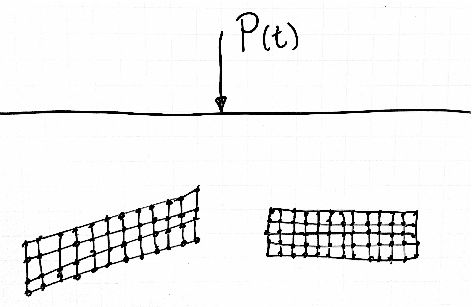
\includegraphics[height=4cm]{img/SGT.pdf}
	\caption{Cálculo de la funciones de Green}
	\vspace{-.5 cm}
\end{figure}
%
%
En cada uno de los $250$ puntos en los que se discretiza la región se aplica un carga unitaria en dos direcciones ortongales, cada carga aplicada es un anális independiente y no se aplica la componente vertical pues dentro de CyberShake no están interesados en esta componente, y se calculan los tensores de deformación de Green sobre los puntos en los cuales se tienen discretizadas todas las fallas para cada una de las cargas.\\
%
Función de Green en Elastodinámica: Desplazamiento debido a una fuente puntual.\\
%
\begin{align*}
	G_{in} \left( \vec{x}, t; \vec{\xi}, \tau \right) \text{Función de Green}
\end{align*}
%
Usando reciprocidad, los Tensores de Deformación de Green se usan para calcular los registros sintéticos en cada uno de los $250$ sitios en los cuales fue discretizada la región para los diferentes escenarios de ruptura que se definieron anteriormente.
%
\begin{figure}[h]
\centering
%%
	\subfloat[Carga 1]{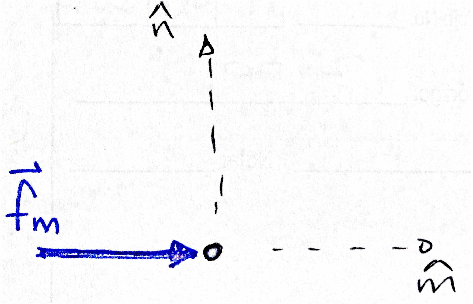
\includegraphics[width=0.4\textwidth]{img/Recipro1.pdf}}\qquad
%	%
	\subfloat[Carga 2]{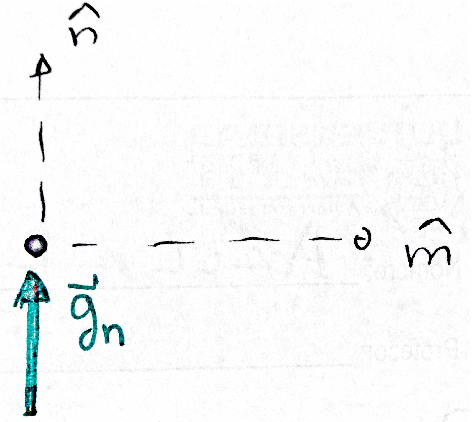
\includegraphics[width=0.4\textwidth]{img/Recipro2.pdf}}
%	%
\caption{Reciprocidad}
%
\end{figure}
%
%
\end{frame}
%
%
\begin{frame}[allowframebreaks]{References}
\def\newblock{}
%\bibliographystyle{gji}
%\bibliography{refSCEC}
\bibliographystyle{plain}
\begin{thebibliography}{1}

\bibitem{book:aki} Keiiti Aki \& Paul G. Richards. {Q}uantitative {S}eismology. University Sciencie Books, 2nd Edition, Mill Valley, San Diego, 2002.

\bibitem{baker} Baker, J. W., Luco, N., Abrahamson, N. A., Graves, R. W., Maechling, P. J., \& Olsen, K. B. (2014, July). Engineering Uses of Physics-based Ground Motion Simulations. In Proceedings of the Tenth US Conference on Earthquake Engineering.

\bibitem{gravesetal} Graves, R.; Jordan, T. H.; Callaghan, S.; Deelman, E.; Field, E.; Juve, G.; ... \& Vahi, K. (2011). CyberShake: A physics-based seismic hazard model for southern California. Pure and Applied Geophysics, 168(3-4), 367-381.

\bibitem{ucerf2} Field, E. H., Dawson, T. E., Felzer, K. R., Frankel, A. D., Gupta, V., Jordan, T. H., ... \& Wills, C. J. (2009). Uniform California earthquake rupture forecast, version 2 (UCERF 2). Bulletin of the Seismological Society of America, 99(4), 2053-2107.

\bibitem{ucerf3} Field, E.H., Biasi, G.P., Bird, P., Dawson, T.E., Felzer, K.R., Jackson, D.D., Johnson, K.M., Jordan, T.H., Madden, C., Michael, A.J., Milner, K.R., Page, M.T., Parsons, T., Powers, P.M., Shaw, B.E., Thatcher, W.R., Weldon, R.J., II, and Zeng, Y., 2013, Uniform California earthquake rupture forecast, version 3 (UCERF3)—The time-independent model: U.S. Geological Survey Open-File Report 2013–1165, 97 p., California Geological Survey Special Report 228, and Southern California Earthquake Center Publication 1792, \url{http://pubs.usgs.gov/of/2013/1165/}.

\end{thebibliography}

\end{frame}


\end{document}

